\documentclass[11pt,letterpaper,twocolumn,english,DIV=calc]{scrartcl}

%%%%%%%%%%%%%%%%%%%%%%%%%%%%%%%%%%%%%%%%%
% This template is based on:
%
% Large Colored Title Article LaTeX Template, Version 1.1 (25/11/12)
% Downloaded from: http://www.LaTeXTemplates.com
% Original author: Frits Wenneker (http://www.howtotex.com)
% License: CC BY-NC-SA 3.0 (http://creativecommons.org/licenses/by-nc-sa/3.0/)
%%%%%%%%%%%%%%%%%%%%%%%%%%%%%%%%%%%%%%%%%

\usepackage{fontspec}
\setmainfont[Ligatures=TeX]{TeX Gyre Heros}
\setsansfont[Ligatures=TeX]{Linux Biolinum O}

\PassOptionsToPackage{svgnames}{xcolor}
\usepackage[
  % HomeHTMLFilename=index, % Filename of the homepage.
  % HTMLFilename={node-}, % Filename prefix of other pages.
  % IndexLanguage=english, % Language for xindy index, glossary.
  % latexmk, % Use latexmk to compile.
	% mathjax, % Use MathJax to display math.
]{lwarp}
% \boolfalse{FileSectionNames} % If false, numbers the files

\makeatletter
\newcommand{\rev}{Revision 6}
\newcommand{\proposed}{{\color{DarkRed}\textsc{(Proposed)} }}
\newcommand{\HorRule}{\color{Black} \rule{\linewidth}{1pt}} % Horizontal rule around the title

\usepackage{draftwatermark}

\usepackage{array}
\usepackage{booktabs} % Horizontal rules in tables
\usepackage[format=plain, labelfont=bf,up, textfont=up]{caption}
\usepackage{enumitem}
\usepackage{fix-cm}	 % Custom font sizes - for the initial letter in the doc
\usepackage{float}
\usepackage{fontawesome}
\usepackage{graphicx}
\usepackage{lastpage}
\usepackage{setspace}
\usepackage{titling} % Allows custom title configuration
\usepackage{units}
\usepackage{url}

\usepackage{lettrine} % Package to accentuate the first letter of the text
\newcommand{\initial}[1]{ % Defines the command and style for the first letter
	\lettrine[lines=2, lhang=0.35, nindent=0.1em, loversize=0.25]{
		\color{DarkRed}{\textsf{#1}}}{}}

\usepackage{tikz}
\usetikzlibrary{arrows,patterns}

\usepackage{polyglossia}
\setdefaultlanguage[variant=american]{english}

\usepackage[footsepline]{scrlayer-scrpage}
\ifoot{\footnotesize\rev}
\cfoot{\footnotesize\copyright\ 2012 - \the\year\ by Phillip Anderson. CC BY-NC-ND}
\ofoot{\footnotesize Page \thepage\ of \pageref{LastPage}} % "Page 1 of 2"
\deffootnote[0.7em]{0pt}{1.6em}{\makebox[0.7em][l]{\textsuperscript\thefootnotemark}}

\usepackage[authoryear]{natbib}
\usepackage[unicode=true, bookmarks=true, bookmarksnumbered=false,
        		bookmarksopen=false, breaklinks=false, pdfborder={0 0 0}, 
	        	pdfborderstyle={}, backref=false, colorlinks=true]{hyperref}
\hypersetup{pdftitle={Polish Horseshoes, Boston Rules},
        		pdfauthor={Phillip Anderson}, pdfsubject={polish horseshoes},
		        pdfkeywords={beer, frisbee, polish, horseshoes, boston}}
\hypersetup{urlcolor=DarkRed, linkcolor=DarkRed}
\pdfstringdefDisableCommands{\def\proposed{\textsc{(Proposed)}}}

\setcounter{secnumdepth}{2}
\setcounter{tocdepth}{2}
\setlist[enumerate, 1]{label=\thesection.\arabic*, parsep=0pt}
\setlist[enumerate, 2]{leftmargin=1.4em}

%%%%%%%%%%%%%%%%%%%%%%%%%%%%%%%%%%%%%%%%%

\pretitle{\vspace{-85pt} \begin{flushleft} \HorRule \fontsize{50}{50}  \color{DarkRed} \selectfont} % Horizontal rule before the title

\title{\textsf{Polish Horseshoes}} % Your article title

\posttitle{\par\end{flushleft}\vskip .0em} % Whitespace under the title

\preauthor{\color{DarkRed} \huge\hspace{2pt}\textsf{Boston Rules}} %

\author{}

\postauthor{\footnotesize \color{Black}
  \hfill \color{Black}\large \rev: \today

  \HorRule\vspace{-50pt}
}

\setlength{\columnsep}{4ex}
\date{}

\makeatother

%%%%%%%%%%%%%%%%%%%%%%%%%%%%%%%%%%%%%%%%%

\begin{document}
\maketitle

\thispagestyle{headings}

\initial{P}olish Horseshoes is a yard game for two in which players take turns throwing a frisbee at their opponent's target and defending their own in an attempt to score or deny points.
Each target consists of an empty bottle perched atop a pole (which may be a clue to the curious appellation).
Players are required to keep one hand occupied with a beverage or a suitable alternative during gameplay, so Polish Horseshoes may be considered a drinking game, but only in the sense that it is very compatible with concurrent imbibing.
Drinking is generally not prescribed or enforced by the rules themselves.

The original game seems to have appeared in the early 2000's, and is now known by a variety of alternate names such as Beersbee, Frisbeener, and Spanish Horseshoes, among others.%
\footnote{\url{http://en.wikipedia.org/wiki/Polish_horseshoes}}
It does not seem to have originated from Poland.
Many variations exist for the rules and, although they are broadly similar on the main points, most descriptions found online are quite vague or over-simplified. 
A game this good needs and deserves a solid, common set of rules.

We first came across Polish Horseshoes late in 2010 via a friend and were immediately hooked. 
\emph{Boston Rules} is our variation of Polish Horseshoes, developed and fine-tuned over the years in and around Boston, Massachusetts. 
It is now a staple of picnics, cookouts, and other outdoor events whenever the weather is agreeable and occasionally even when it is not. 
Described here are our official rules, recommendations for equipment, and suggestions for playing safely. 
We hope you enjoy the game as much as we have.


\part*{Equipment}

Only a few bits are needed to play, most of which are easily acquired.
Here is the essential equipment list with specific recommendations. 

\begin{description}[font=\large, leftmargin=0.5em]
	\item [{Aerobie® Superdisc™:}] 
		The weight, control, and soft edge of these discs make them ideal for play.%
		\footnote{\href{http://www.aerobie.com/products/superdisc.htm}{Aerobie® Superdisc™}} 
		Lighter discs tend to be cheap and difficult to control. 
		Heavier discs or those with hard edges are prone to destroying bottles very quickly.
		\begin{figure}[h]
			\centering{}
			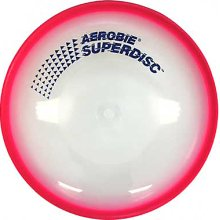
\includegraphics[width=0.25\textwidth]{images/superdisc}{\footnotesize{}

			Source:
			\href{http://www.aerobie.com}{aerobie.com}}		
		\end{figure}
	\item [{Poles (2):}]
		A pair of $1.2\,\mbox{m}$ ($48"$) ski poles is typically used, but anything with a pointy end for the ground and a cap on which to balance a bottle is a potential substitute.
    Tennis balls can (optionally) be fit onto the top to create a ball-and-socket joint if the plastic cups fit. 
	\item [{Plastic cups (2+):}] 
		Common $450\,\mbox{mL}$ ($16\,\mbox{oz.}$) cups work well and are easy to find.
		These are inverted and placed on the poles to provide a platform for the bottles. 
		Keep tape or extra cups on hand, since the cups often crack and break.
	\vfill
	\item [{Empty Bottles (2):}] 
		Ordinary $355\,\mbox{mL}$ ($12\,\mbox{oz.}$) glass bottles can be used but are hazardous due to the potential of shattering during play.
		Do not use glass bottles if you are uncomfortable with the prospect of sharp objects flying towards your hands and face, or if the environment is inappropriate (i.e., public parks and beaches).

		Filling bottles with expanding polyurethane foam reduces the risk of breaking for a negligible increase in weight, but the safest solution is to use plastic bottles loaded with foam and weights to mimic the weight and balance of a standard bottle. 
		These are typically marketed and sold as shooting targets.%
		\footnote{\href{https://gosportsoutdoors.com/products/gosports-outdoors-blast-bottles-6-pack-shatterproof-bottle-shooting-targets-with-rope-for-firearm-target-practice}{GoSports Blast Bottles}}
		\begin{figure}[h]
			\centering{}
			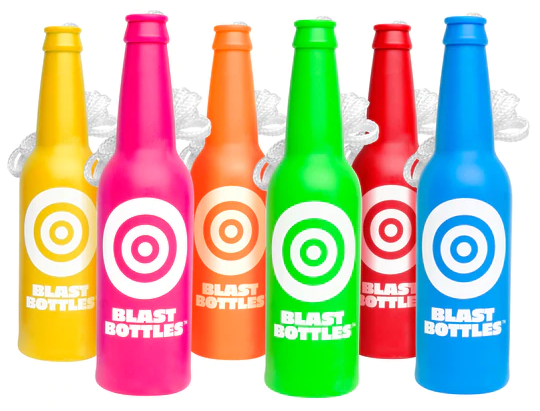
\includegraphics[width=0.4\textwidth]{images/blastbottles}{\footnotesize{}

			Source:
			\href{https://gosportsoutdoors.com}{gosportsoutdoors.com}}
		\end{figure}
		
	\item [{Tasty~beverages:}] 
		All players will need a tasty beverage of their choice, or equivalent, to occupy one hand during play. 
		Glass vessels are at risk of shattering if hit, so aluminum cans are recommended.
\end{description}
\vfill

\begin{figure*}[hpbt!]
	\begin{centering}
		%\usetikzlibrary{arrows,patterns}
\begin{tikzpicture}[line cap=round,line join=round,>=stealth,x=1.1cm,y=1.1cm]

% court specifications
\def\w{2.5} % width of court
\def\pp{10} % minimum pole to pole distance
\def\d{2.5} % depth of player area
\def\pzi{0.4} % depth that pole zone is inset into player area
\def\pzw{1.6} % width of pole zone
\def\pzd{0.5} % depth of pole zone
\def\extra{0.5} % how much to extend guide lines
\def\bt{0.1} % border thickness for player area

% convenience definitions
\def\hw{\w/2} % half the width of the court
\def\hpp{\pp/2} % half the minimum pole to pole distance

% entire court area
\draw[fill=green!25] (-\hpp+\pzi-\d,-\hw) rectangle (\hpp-\pzi+\d,\hw);

\foreach \i in {-1,1}{
  % player zones
  \draw[fill=brown] ({\i*(\hpp-\pzi)}, -\hw) rectangle ++(\i*\d, \w);
  \draw[fill=brown!20] ({\i*(\hpp-\pzi+\bt)}, -\hw+\bt) rectangle ++({\i*(\d-2*\bt)}, \w-2*\bt);
}

% pattern for middle zone
\fill[pattern=crosshatch dots, pattern color=black!40] 
	(-\hpp-\pzd/2,-\hw) rectangle (\hpp+\pzd/2,\hw);

% half court line and label
\draw[dashed] (0,-\hw) -- (0,\hw+\extra/2) node[above] {half court};

\foreach \i in {-1,1}{
  % pole zones
  \draw[rounded corners=5*\pzd, fill=yellow!30] (\i*\pp/2,-\pzw/2) rectangle ++(\i*\pzd,\pzw);
    
  % bottles
  \draw[color=red, fill=red] ({\i*(\hpp+\pzd/2) +\i*0.08}, rand/3) circle(.1) coordinate(cup);
  \draw[thin, color=black,fill=brown] (cup) circle (0.08) circle(0.03);

  % bottle plane lines and labels
  \draw[dashed] ({\i*(\hpp+\pzd/2)},0) +(0,-\hw) -- +(0,\hw+\extra/2) node[above] {$bp$};
  \draw[dashed] (\i*\hpp, -\hw-\extra/2) -- ++(0, \hw);
}
\draw[dashed] (\hpp+\pzd, -\hw-\extra/2) -- ++(0, \hw);

% distance callouts for middle zone, court width, pole zone depth, and player area depth, respectively
\draw[thick,|<->|] (-\hpp, -\hw-\extra) -- node[fill=white] {\pp\ m} +(\pp,0);
\draw[thick,|<->|] (\hpp-\pzi+\d+\extra,-\hw) -- node[fill=white, xshift=7] {\w\ m} +(0,\w);
\draw[thick,|<-] (\hpp+\pzd,-\hw-\extra) -- node[fill=white, anchor=west, xshift=0] {\pzd\ m} +(\pzd,0);

% \draw[thick,|<->|] (\pp/2,-\w/2-2*\extra) -- node[fill=white, anchor=north, yshift=-5] {\pzd\ m} +(\pzd,0);
% \draw[thick,|<->|] (\pp/2+\pzd,-\w/2-\extra) -- node[fill=white] {\sim\d\ m} +(\d,0);
% \draw (0,0) circle(1);

%players left (top, bottom) and right (top, bottom)
\begin{scope}[thick, x=2mm, y=2mm, xshift=-7cm, xscale=1, rotate=-20]
	\draw[line width=1.8mm] (0, 1.65) -- ++(0.8, .4) -- ++(1.2, 0.1) coordinate(hand1);
	\draw[color=black!20!red,line width=1.3mm] (0, 1.65) -- ++(0.8, .4) -- ++(1.2, 0.1);
	\draw[line width=1.8mm] (0, -1.65) -- ++(.5, -.5) -- ++(.7, -.3) coordinate(beer1);
	\draw[color=black!20!red, line width=1.3mm] (0, -1.65) -- ++(.5, -.5) -- ++(.7, -.3);
	\draw[thin, fill=brown!60] (hand1) ellipse(0.5 and 0.4) (beer1) ellipse(0.6 and 0.4);
	\draw[thin, fill=brown] (beer1) +(0,0.3) circle(0.45) circle(0.18);
	\draw[fill=red] ellipse(.8 and 2);
	\draw[fill=brown!50!black] (.1,0) circle(1);
\end{scope}
\begin{scope}[thick, x=2mm, y=2mm, xshift=7cm, xscale=-1, rotate=-20]
	\draw[line width=1.8mm] (0, 1.65) -- ++(0.8, .4) -- ++(1.2, 0.1) coordinate(hand1);
	\draw[color=blue!60,line width=1.3mm] (0, 1.65) -- ++(0.8, .4) -- ++(1.2, 0.1);
	\draw[line width=1.8mm] (0, -1.65) -- ++(.5, -.5) -- ++(.7, -.3) coordinate(beer1);
	\draw[color=blue!60, line width=1.3mm] (0, -1.65) -- ++(.5, -.5) -- ++(.7, -.3);
	\draw[thin, fill=brown!60] (hand1) ellipse(0.5 and 0.4) (beer1) ellipse(0.6 and 0.4);
	\draw[thin, fill=brown] (beer1) +(0,0.3) circle(0.45) circle(0.18);
	\draw[fill=blue!70] ellipse(.8 and 2);
	\draw[fill=brown!50!black] (.1,0) circle(1);
\end{scope}

\end{tikzpicture}
\vspace{-5mm}\par
	\end{centering}
	\caption{
		Top-down schematic of the court. 
		Poles (brown dots) can be placed anywhere within the pole zones (yellow regions). 
		Players stand behind the \emph{bottle plane} ($bp$) on their respective side.\label{fig:court}
	}
\end{figure*}

\pagebreak
\part*{Court}%

A polish horseshoes court is composed of a \mbox{$10\textrm{ m}\times2.5\textrm{ m}$} clearing bookended by $0.5\,\mbox{m}$ wide pole zones and player boxes, as shown in figure~\ref{fig:court}.
Edges of the court do not prescribe bounds but may be marked by physical boundaries such as fences or walls.
In fact, there are no bounds \emph{per~se}, but areas deemed particularly undesirable for the disc to hit or land in (e.g., windows, bodies of water, rough terrain, neighbors' yards) are designated as \emph{traps}.

The court should be free of traps, but low obstructions and uneven terrain are allowed in the central area.
Player boxes must be clear, reasonably flat, and at a similar elevation to each other.
\emph{Breakers} such as rocks or other hard objects may be located along the perimeter.
Pole zones should contain a packable dirt or clay mixture so that the poles are easily planted and supported.

Players face each other from their respective boxes on opposing ends of the court and set their poles.
This is done by planting the pole anywhere in the pole zone, placing an inverted plastic cup over the cap to form a flat base, and balancing an empty bottle on top, as shown in figure~\ref{fig:pole-setup}. 
The cup is considered to be part of the pole.
 
Players position themselves behind their own \emph{bottle plane}, an imaginary plane perpendicular to the long axis of the court that extends vertically from the ground through the point of the bottle closest to half court.  
When defending, if the disc approaches below the top of the bottle, the $bp$ is shifted forwards or backwards to intersect the leading edge of the pole or bottle at the height of the disc as shown in figure~\ref{fig:pole-setup}.

\begin{figure}[!hbtp]
	\begin{centering}
		\begin{tikzpicture}[line cap=round,line join=round,>=stealth,x=1mm,y=1mm]

\def\ch{10} %cup height
\def\cdt{8} %cup top diameter
\def\cdb{6.0} %cup bottom diameter

\def\pl{70} %pole length actually 120
\def\pt{7.5} %pole taper length
\def\pd{1.6} %pole diameter
\def\dd{5} %disc diameter
\def\dt{1.9} %disc thickness
\def\balld{6.0} %tennis ball diameter
\def\extra{4} %how much to extend guide lines

\begin{scope}[xshift=0mm,scale=.55]

\draw[rotate=-10] (0,\pl-2) coordinate (B);

%ground
\draw[fill=brown,color=brown] (-4*\extra,-3*\extra) rectangle (32*\extra,0);
\draw[ultra thick, color=black!30!green] (-4*\extra,0) -- (32*\extra,0);
\draw[->, thick] (29*\extra, 2*\extra) node[left] {half court} -- (31*\extra, 2*\extra);

%cup
\draw (B) ++(0, \dt/2+2.5) coordinate(cup);
\draw[red,fill=red!10, thick] (cup) ++(-\cdt/2,-\ch) -- ++(\cdt/2-\cdb/2,\ch) -- ++(\cdb,0) -- ++(\cdt/2-\cdb/2,-\ch) -- cycle;
\draw[black,fill=white,thin] (cup) ++(-\cdt/2,-\ch-.3) rectangle ++(\cdt,.6);
\draw[black,fill=white,thin] (cup) ++(-\cdt/2,-\ch) circle (.5) ++(\cdt,0) circle (.5);

%pole
\begin{scope}[rotate=-10]
\draw[fill=yellow] (-\pd/2,0) rectangle ++(\pd,\pl); %pole
\draw[fill=black] (-\pd/2,\pl) rectangle ++(\pd,-\pl/10); %handle
\draw[fill=gray] (0,-\pt) -- ++(-\pd/2,\pt) -- ++(\pd,0) -- cycle; %spike
\draw[fill=white] (-2*\pd,-0.5) rectangle (2*\pd,0.5); %guard
\draw[fill=green] (B) circle (\balld/2); %tennis ball
\end{scope}

%bottle
\begin{scope}[scale=.25]
\draw[fill=black!50!brown] 
(cup) ++(0,1)
 .. controls ++(-1,0) and ++(1,0) .. ++(-6.6,0)
.. controls ++(-3.2,0.2) and ++(0,-2.5) .. ++(-5.8, 4.2)
.. controls ++(0,1) and ++(0,-1) .. ++(0,47.2)
.. controls ++(0,2.5) and ++(-0.9,-1.4) .. ++(2.3,5.7)
.. controls ++(1.9,3.1) and ++(-0.3,-1.4)   .. ++(2.6,5.3)
 .. controls ++(0.5,2.1) and ++(-0.9,-16.8)  .. ++(1.9, 25.6) 
 .. controls ++(-0.4,0.4) and ++(-0.2,-1.1)  .. ++(-0.2, 3.3)
 .. controls ++(0.2,0.5) and ++(0.2,-0.2)  .. ++(-0.1,1.3) 
.. controls ++(-0.6,0.9) and ++(-1.1, -0.4)  .. ++(1.2,3.5) 
.. controls ++(1.2,0.4) and ++(-2.2,0)  .. ++(4.7, 0.2)

.. controls ++(2.2,0) and ++(-1.2,0.4) .. ++(4.7, -0.2)
 .. controls ++(1.1, -0.4) and ++(.6,0.9) .. ++(1.2,-3.5) 
 .. controls ++(-0.2,-0.2) and ++(-0.2,0.5) .. ++(-0.1,-1.3) 
 .. controls ++(0.2,-1.1) and ++(0.4,0.4) .. ++(-0.2, -3.3)
 .. controls ++(0.9,-16.8) and ++(-0.5,2.1) .. ++(1.9, -25.6) 
.. controls ++(0.3,-1.4) and ++(-1.9,3.1) .. ++(2.6,-5.3)
.. controls ++(0.9,-1.4) and ++(0,2.5) .. ++(2.3,-5.7) 
.. controls ++(0,-1) and ++(0,1) .. ++(0,-47.2)
.. controls ++(0,-2.5) and ++(3.2,0.2) .. ++(-5.8, -4.2) 
.. controls ++(-1,0) and ++(1,0) .. ++(-6.6,0)
;

% bottle planes
\draw[dashed, red, very thick] (10,0) -- ++(0, 450) node[above] {A};
\draw[dashed, blue, very thick] (35,0) -- ++(0, 450) node[above] {B};
\draw[dashed, orange, very thick] (62,0) -- ++(0, 450) node[above] {C};

% discs
\draw[dotted, red, thick] (10, 45) -- (180, 45);
\draw[red, fill=red] (180, 45) -- ++(8, 12) -- node[above] {A} ++(100, 0) -- ++(8, -12) -- cycle;

\draw[dotted, blue, thick] (35, 180) -- (200, 180);
\draw[blue, fill=blue] (200, 180) -- ++(8, 12) -- node[above] {B} ++(100, 0) -- ++(8, -12) -- cycle;

\draw[dotted, orange, thick] (62, 410) -- (220, 410);
\draw[orange, fill=orange] (220, 410) -- ++(8, 12) -- node[above] {C} ++(100, 0) -- ++(8, -12) -- cycle;
\end{scope}
\end{scope}
\end{tikzpicture}

\vspace{-5mm}\par
	\end{centering}
	\caption{
		Pole setup. 
		Pointy end in the ground. 
		An inverted plastic cup covers the cap, creating a flat base for the bottle. 
		Round caps form a ball-and-socket joint with the cup and allow the bottle to be balanced even when the pole is not vertical.
		The $bp$ may shift when defending according to the height of the incoming disc. Vertical dashed lines \textcolor{red}{A}, \textcolor{blue}{B}, and \textcolor{orange}{C} indicate the bottle plane for the corresponding three incoming throws.
		\label{fig:pole-setup}
	}
\end{figure}

\clearpage
\part*{Gameplay}

This section describes the rules for a \emph{singles} game.
\emph{Doubles} games and all other variations are based on these foundational rules.
Refer to the \nameref{part:variants} section for applicable rule adjustments.
	
\section{Basic play and terminology}
\begin{enumerate}
	\item All players must have a tasty beverage or equivalent in one hand during play.
	\item Both players start with 0 points (pts) and 10 HP.
	\item \label{enu:fair_toss} The winner of a fair toss chooses to have first throw or preferred side.
	\item \label{enu:alternate_throws} Players alternate throwing the disc, which is \emph{live} at the point of release and \emph{dead} upon contacting any object afterwards.

	\item The disc is considered \emph{catchable} if it crosses the $bp$ (i) between the defender's knees and hairline, and (ii) within $1\,\mbox{m}$ to either side of the Defense's bottle, subject to some exceptions.
	\begin{enumerate}
		\item The disc is not catchable if it is within one diameter of an obstacle when it crosses the bottle plane (safety exception).
		\item The disc is not catchable if it lands within one diameter behind the $bp$ (steep throw exception).
	\end{enumerate}

	\item The disc is \emph{short} if it comes to rest without crossing the $bp$. 
		Offense has the option to throw a shorted disc from its resting position. 

	\item Catching, blocking, or deflecting a live disc before it breaks the $bp$ is \emph{goaltending}.
	
	\item The disc \emph{hits} if it makes contact with the opponent's pole or bottle, otherwise it \emph{misses}.
	A hit is \emph{direct} if the disc is not dead before contactin the pole or bottle, and \emph{grazing} if it does not result in the bottle falling.

\end{enumerate}

\section{Scoring}
\begin{enumerate}
	\item \label{enu:dropped_point}Offense is awarded 1\,pt for throwing a live catchable miss that is not caught (\emph{dropped}).
	\item \label{enu:bottle-hit}Offense is awarded 1\,pt for a direct bottle hit.
	\item Offense is awarded 2 pts for any hit that results in the Defense's bottle touching the ground.
	\item \label{enu:stalwart}Defense is awarded one point for catching the disc and the bottle before either touch the ground after a live non-grazing hit (\emph{stalwart defense}). 

	\item If a throw is goaltended, Offense is awarded points corresponding to the most likely hit.
	\begin{enumerate}
		\item If the goaltender does not have both feet behind the $bp$, Offense is awarded a minimum of two points (\emph{man-in-the-middle attack}).
	\end{enumerate}

	\item Points are not awarded for dropped discs, hitting the bottle, or performing a stalwart defense if they would result in a victory (i.e. rules \ref{enu:dropped_point}, \ref{enu:bottle-hit}, and \ref{enu:stalwart} are suspended). Instead, the opponent loses the equivalent in HP.

	\item All rules and penalties stack.
	\item Points and penalties are resolved in the order of occurrence, not simultaneously per play.
\end{enumerate}

\section{Winning the game}
There are three ways to end the game.
\begin{enumerate}
	\item \label{enu:win-conditions}Point victory: Play goes to 11\,pts, win by two.
		Above 11, players are either tied (\emph{deuce}) or one leads by a single point (\emph{advantage}).
		\begin{enumerate}
			\item Play does not end upon loss of a point (see sections \ref{subsec:clumsiness-and-carelessness} and \ref{subsec:traps} for scenarios), even if the conditions in rule \ref{enu:win-conditions} are met, but the penalized player may become \emph{profoundly disadvantaged} or worse under these circumstances.
		\end{enumerate}
	
	\item Not-so-sudden-death: If a player reaches 0 HP, they lose the game.

	\item Fatality: If a bottle cracks or breaks, the owning player loses the game.
	\begin{enumerate}
		\item A bottle with only one crack, which does not extend below the shoulder, may be replaced but not defended for the remainder of the game (\emph{ghost bottle} exception).
		\item A cracked ghost bottle cannot be replaced (\emph{no more continues} exception).
	\end{enumerate}
\end{enumerate}

\section{\label{sec:special-scenarios}Special scenarios}

\subsection{\label{subsec:clumsiness-and-carelessness}Clumsiness and carelessness}
\begin{enumerate}[leftmargin=2.8em, label=\thesubsection.\arabic*]
	\item If a player steps over the $bp$ while throwing, no points are awarded for the play (\emph{line fault}). 
	If this throw results in a broken or damaged bottle, the bottle is replaced.
	
	\item If a player allows their tasty beverage to suffer a hit from a live disc, they lose 1\,pt.
	\item If a player drops their tasty beverage, they lose 1\,pt.
	\item If a player grabs an undisturbed bottle, they lose 1\,pt.
	\item If a player disturbs their own pole or bottle and the bottle hits the ground, the opponent is awarded 2 or 3\,pts, respectively.
	This excludes drops when resetting.
	\item If a bottle hits the ground as a result of a player disturbing their own pole or bottle, the opposing player is awarded 2 or 3\,pts, respectively.
	This does not apply during resets.
	\item If a player throws with their bottle unset, they lose 1\,pt if the bottle is not reset before the return throw.
	\item Points and penalties are not awarded for \emph{acts of god}, such as strong gusts.
\end{enumerate}

\subsection{\label{subsec:traps}Traps and redemption shots}
\begin{enumerate}[leftmargin=2.8em, label=\thesubsection.\arabic*]
	\item The default penalty for throwing the disc into a trap is the loss of 1\,pt, but more severe penalties can be set, including loss of game.
	\item The thrower is responsible for retrieving the disc from a trap when retrieval is difficult.
	\item The thrower may throw a trapped disc from its resting position if there is no line of sight to the opponent's bottle (\emph{redemption shot}). 

	\begin{enumerate}
		\item Redemption shots can not be defended.
		\item If the shot knocks the opponent's bottle to the ground, the thrower regains 1\,pt.
		\item If the disc lands in a trap, the thrower is further penalized for that trap.
		\item Redemption shots can not be chained.
	\end{enumerate}
\end{enumerate}

\subsection{On fire}
\begin{enumerate}[leftmargin=2.8em, label=\thesubsection.\arabic*]
	\item \label{enu:fire_count} A player who executes three consecutive direct hits is \emph{on fire}.
	The player is \emph{heating up} after the second hit.
	\item Normal play is suspended while a player is on fire. 
	The on fire player throws until failing to make a direct hit, at which point fire is lost and that player's fire count returns to zero.
	\item Fire throws cannot be defended, the bottle may not be caught, and points are awarded as if in normal play.
	\item \label{enu:splooshing_1} Consecutive hit count for a player is \emph{splooshed} (reset to zero) if the opposing team makes a 2+\,pt play.
	\item Consecutive hit count for a player is reset to zero if that player's tasty beverage suffers a direct hit.
	\item Goaltending does not affect any player's fire count.
	\item Ambiguities in \emph{fire} rules may be settled by an appeal to NBA Jam.
\end{enumerate}

\subsection{Extreme events and beverage debts}
\begin{enumerate}[leftmargin=2.8em, label=\thesubsection.\arabic*]
	\item A \emph{shutout} occurs when the loser does not have a positive score at the end of a game.

	\begin{enumerate}
		\item All losers of a shutout must drink an agreed upon \emph{nasty beverage}.
		\item An additional drink is owed for each point the \emph{loser}'s score is below zero.
	\end{enumerate}

	\item \emph{Shooting the moon} occurs when the winner does not have a positive score at the end of a game (by breaking the opponents bottle).

	\begin{enumerate}
		\item The loser of a moon shot must drink an agreed upon \emph{nasty beverage}.
		\item The loser owes a nasty beverage for each point the \emph{winner's} score is below zero.
	\end{enumerate}

	\item \emph{Mutual shame} occurs if neither team has a positive score at the end of a game.

	\begin{enumerate}
		\item All victims of mutual shame must drink a nasty beverage.
		\item Debts from mutual shame may not be wagered, forgiven, canceled, or transferred.
	\end{enumerate}

	\item A \emph{photo-finish} occurs when both teams are tied at the end of a game.
	\item The nasty beverage should be chosen before the game begins.

	\begin{enumerate}
		\item The choice of nasty beverage may be agreed upon or changed at any time if the players involved agree on the new choice.
		\item If players cannot come to an agreement, the default beverage choices are Bud Light with Lime, Smirnoff Margarita, or PBR with a fresh squeezed lime.
		\item Debts from a moon shot may be settled with any moon-themed shot or beverage.
	\end{enumerate}

	\item Unless otherwise specified, beverage debts do not have to be repaid immediately and they may be wagered, forgiven, canceled, or transferred (by trickery if necessary). 
	\item Beverage debts may be reduced if paid in bulk, at the discretion of the parties owed.
\end{enumerate}

\section{Series and tournament play}
\begin{enumerate}[label=\thesection.\arabic*]
	\item In regular season and tournament play, the winner of a \emph{match} must win the majority of sets in a best-of-M format (M typically 1). Sets are won by winning the majority of games in a best-of-N format (N typically 3).
	\item Player sides and first throw alternate every game of the match after the first.
	Rule~\ref{enu:fair_toss} is applied to initiate the match.
	
	\item Each team must use the same bottle for the duration of a match.

	\begin{enumerate}
		\item A broken bottle is replaced for the next game. 
		Replacements must be used for the rest of the match or until they break.
	\end{enumerate}
	\item \proposed Each player may be alloted a fixed number of bottles for the season
	\item \proposed Handicap system for series play.

\end{enumerate}

\newpage
\part*{Box Scoring System}
Section stub for a description of the scoring shorthand.

\part*{Variants}
\label{part:variants}

Variants are based on the rules for a singles game. Rules listed here extend the base rules where there is no conflict, and supersede where there is.

\section{Doubles}
Four players face off, with the pairs on either side of the court forming a team. 

\begin{description}
	\item{\S\ref{enu:alternate_throws}} Teams and teammates alternate throws. 
	\item{\S\ref{enu:dropped_point}} Offense is also awarded one point for throwing a live hit if the disc is uncaught.
	\item{\S\ref{enu:win-conditions}} Play goes to twenty-one points, win by two.
	\item{\S\ref{enu:fire_count}} Fire counts are tracked per player and not per team.
\end{description}

\section{Di-Polish \proposed}
Each player has two poles and bottles.

\section{Standard Polish \proposed}
Each side has a \emph{battle standard} behind their bottle plane and to one side of the court.

% \section{Glossary}
% Sukes Angle
% Gentlemen's Timeout
% Can cup

\newpage

\part*{Back Matter}

\addsec{Credits}

Many thanks to everybody who helped with game development and codifying the rules (in alphabetical order):\medskip{}

\begin{tabular}{>{\raggedright}p{3.5cm}>{\raggedright}p{2.5cm}}
	Phillip Anderson & Julian S.\tabularnewline
	Mike C. & Jon S.\tabularnewline
	Will E. & Konrad S.\tabularnewline
	Mike F. & Matt T.\tabularnewline
	Jon K. & Kristine W.\tabularnewline
	Andrew O. & Dustin W.\tabularnewline
\end{tabular}

\addsec{Disclaimer}

Nobody involved with writing or distributing this document is responsible for injuries that may be caused by playing this game.

\medskip{}\noindent Polish Horseshoes is not sponsored or endorsed by any of the companies mentioned.

\addsec{License}

\copyright\ 2012 - \the\year\ by Phillip Anderson. 

\noindent This work is licensed under the Creative Commons Attribution
- NonCommercial - NoDerivatives 4.0 International License. 
Visit \href{http://creativecommons.org/licenses/by-nc-nd/4.0/}{creativecommons.org} to view a copy of this license.

\begin{figure}[!ht]
	
\includegraphics[width=\columnwidth]{images/by-nc-nd}
\end{figure}

\newpage{}

\ \vfill{}

\noindent Visit, contact or follow at the following links for questions, comments, or other communications:

\begin{description}[listparindent=1.cm, font=\normalfont]
	\item[{\faGlobe}] \href{https://github.com/anderson-pa/polish_horseshoes/releases}{https://github.com/anderson-pa/\\\indent polish\_horseshoes/releases}

	\item[\faEnvelopeO] \href{mailto:brpolish@gmail.com}{brpolish@gmail.com}

	\item[\faTwitter] \href{http://www.twitter.com/br_polish}{@br\_{}polish}

	\item[\faTwitch] \href{http://www.twitch.tv/br_polish}{br\_{}polish}
\end{description}

\end{document}
